\begin{figure}
    \begin{enumerate}
        \item[(a)] 
\includegraphics[scale=1.02]{plot_relaxed_similarity_papertop.pdf}\\
        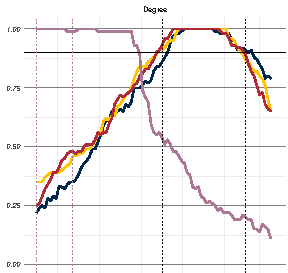
\includegraphics[scale=1.02,trim={0 0.8mm 0 0},clip]{plot_relaxed_similarity_paper_degree.pdf}\hspace*{0.2mm}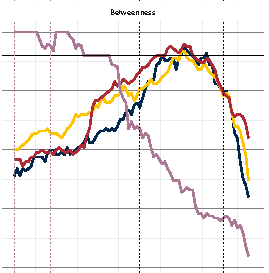
\includegraphics[scale=1.02,trim={0 0.3mm 0 0},clip]{plot_relaxed_similarity_paper_betweenness.pdf}\hspace*{-0.45mm}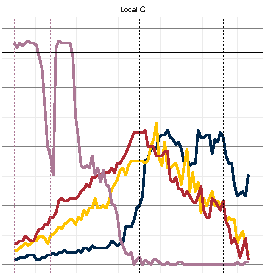
\includegraphics[scale=1.02,trim={0 0.8mm 0 0},clip]{plot_relaxed_similarity_paper_localc.pdf}\\
        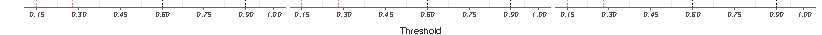
\includegraphics[scale=1.02]{plot_relaxed_similarity_paperbottom.pdf}
        \vspace*{-0.6cm}
        \item[(b)] \hspace*{-0.25cm}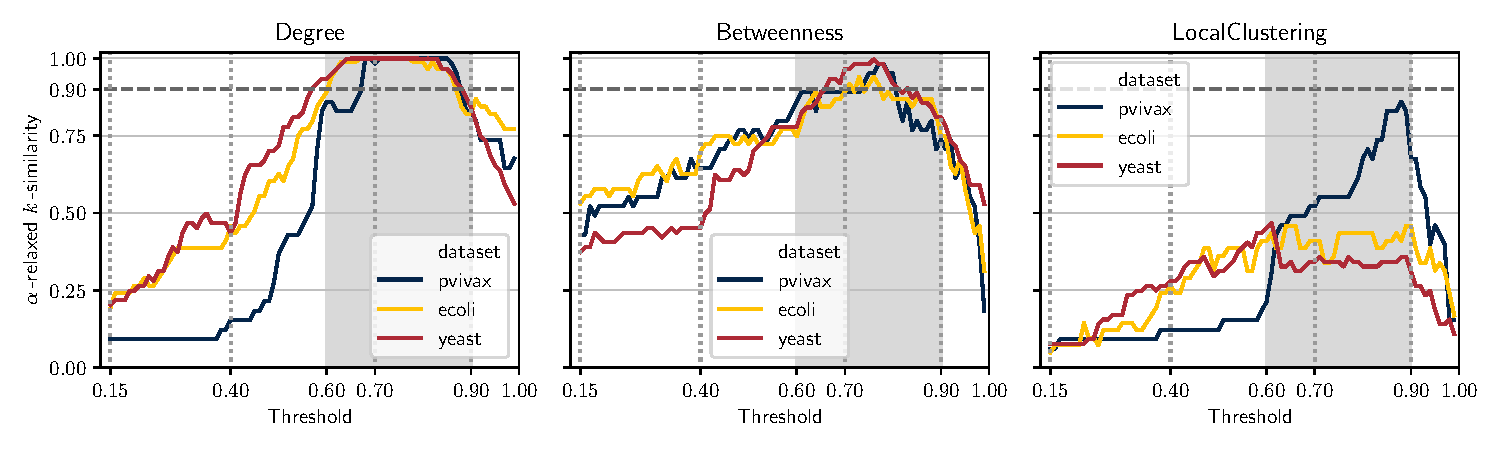
\includegraphics[align=t,width=0.97\linewidth]{plot_relaxed_similarity_graffs.pdf}
    \end{enumerate}
    \vspace*{-0.6cm}
    \caption{$\alpha$-relaxed $k$-similarity plots between overall rank and ranks at individual thresholds, taking results from The Paper~(a) and \graffs~(b).
    The overall rank for each of 3 metrics was calculated within the ``wide medium-high confidence region'' $\left[ 0.6, 0.9 \right]$, and $\alpha$ was set to $1.5$.}
    \label{fig:plot_relaxed_similarity}
    %\footnotetext{Chosen according to \url{https://github.com/lbozhilova/measuring_rank_robustness/blob/master/robustness_analysis_aux.R#L108}}
\end{figure}
